\begin{figure}[tbp] 
  \centering
  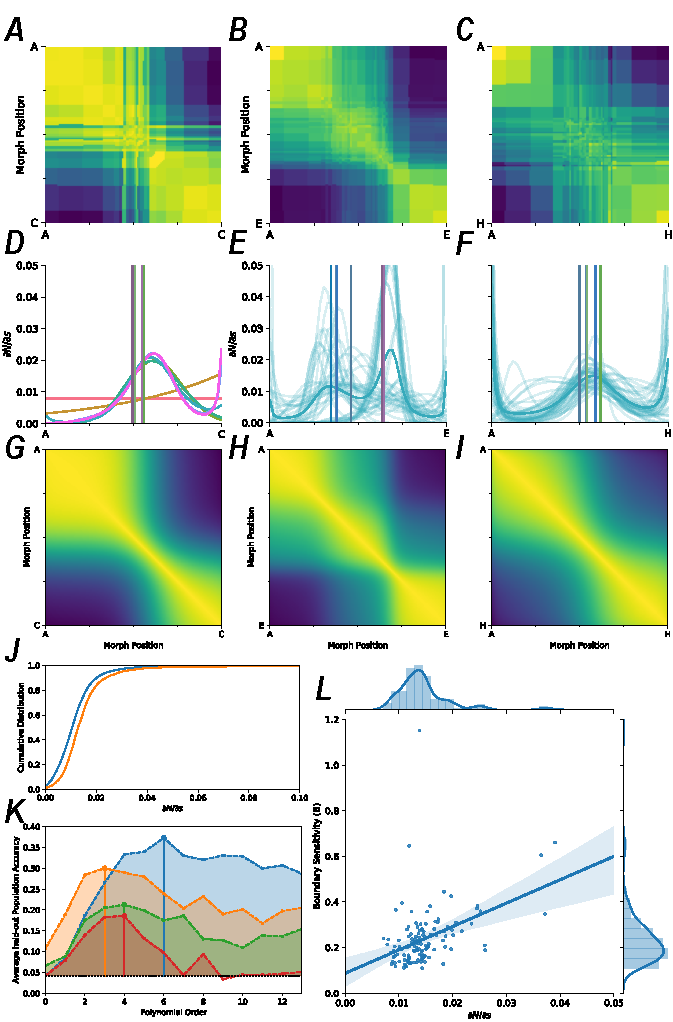
\includegraphics[width=114mm]{figures/fig07_derivative.pdf}
  \caption[The \Thielk curve captures how neural representation changes as we move along a morph dimension]
{(continued on following page.)
\index{derivative}}
  \label{fig:derivative}
\end{figure}

\begin{figure}[tp]
  \contcaption{
(A)	The cross correlation matrix for a single recording on the morph dimension from motif A to motif C. Average cosine distance in the task relevant neural representation subspace between pairs of morph positions are initially calculated. These values are then upsampled to the full 128 pixel grid using nearest neighbor interpolation.
(B-C)	Average cross correlation matrix for all recordings (using the final stimuli set) for morph dimensions A to E and A to H.
(D)	Using a polynomial of order 0 through 6 to estimate the \Thielk curve for a single recording and morph dimension, A to C (same as above).
Vertical lines represent the behaviorally determined psychometric boundaries for all birds tested across this morph dimension. The horizontal pink line is the 0th order fit, the exponential gold line is the 1st order fit.
(E-F)	4th order mean \Thielk curves across all recordings on morph dimension AE (E) and AH (F). Individual 4th order \Thielk curves for each recorded population are faintly plotted to show variance. Vertical lines represent the behaviorally determined psychometric boundaries for all birds tested across this morph dimension.
(G)	Cross correlation matrix reconstructed from the 4th order \Thielk curve for the same recording used in (A) and (D).
(H-I)	Average reconstructed cross correlation matrix from all 4th order \Thielk curves on AE (H) and AH (I)
(J)	Cumulative distributions of the value of the 4th order \Thielk curve at psychometric boundary locations of the same dimension vs different dimensions as a control. A one-sided KS test provides a P value of $p=1.47E-121$
(K)	Average accuracy of predicting the morph dimension of a \Thielk curve from a held out recorded neural population as we increase the order of the polynomial. The green and orange curves use the optimized polynomial coefficients to predict the morph dimension label. The red and blue curves use the normalized \Thielk curve evaluated at 50 evenly spaced points along the morph dimension. The red and green curves use a multinomial logistic regression as the classification model. The orange and blue curves use XGBoost as the classification model. The vertical lines highlight the maximum average held-out prediction accuracy achieved by each method. Chance performance ($1/24$) plotted as a horizontal dotted line.
(L)	Correlation between the boundary sensitivity parameter (B) of the psychometric curve and the value of the 4th order \Thielk curve for the given boundary location. Plotted above and to the right are the projected histograms and associated kernel density estimate of the distribution. Plotted as a line is the regression between these two variables with 1000 fold bootstrapped 95\% confidence interval plotted as a shaded region around the regression.
}
\end{figure}